\chapter{Valutazione e test}

\section{Test delle funzionalità}

In primo luogo è stato verificato il buon comportamento delle singole parti grazie all'ispezione dei diagrammi d'onda prodotti dalla simulazione. In secondo luogo il programma VHDL è stato sottoposto a quattro test bench per verificare la correttezza dei risultati.

\subsection{Funzionalità}
la figura \ref{fig:io} mostra una sequenza di lettura dell'intestazione e scrittura del risultato. Come spiegato in sezione \ref{io} e illustrato in figura, i segnali in ingresso alla memoria ($o \textunderscore adress$, $o \textunderscore en$, $o \textunderscore we$, $o \textunderscore data$) sono mantenuti stabile tra due fronti di discesa del clock per garantire la corretta lettura o scrittura del dato che avviene sul fronte di salita. La memoria assegna quindi il valore al segnale $i \textunderscore $ sul fronte di salita mentre il componente lo utilizza nel successivo periodo basso del clock per garantire un tempo delta di salvaguardia prima dell'utilizzo per il suo aggiornamento.\\

Gli indirizzi letti sono correttamente 2, 3, 4 e quelli scritti 1, 2. I valori letti sono in esadecimale: il numero di colonne, pari a 18, quello di righe, uguale a 7, e il valore di trigger $ff$.

\begin{figure}
	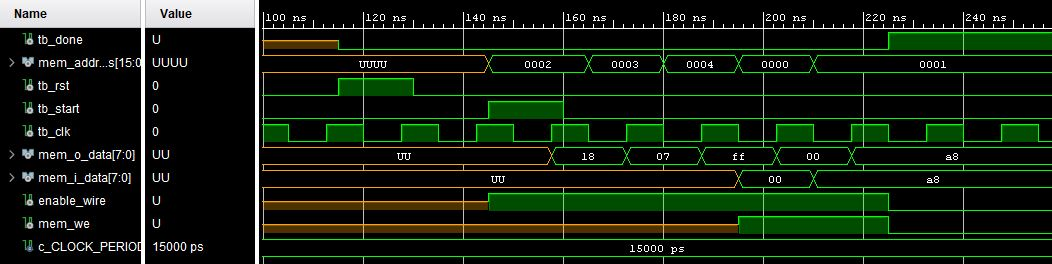
\includegraphics[scale=0.5]{evaluation/IO.JPG}
    \caption{capture of the siulation wave diagram }
    \label{fig:io}
\end{figure}

\subsection{Test bench}
I quattro test effettuati usano l'immagine rappresentata in figura \ref{file} con quattro diversi livelli di colori di interesse: 255, 0, 2 e 21 rispettivamente.\\
I risultati attesi (0, 168, 110 e 21 rispettivamente) sono correttamente riscontrati.\\

\begin{figure}
	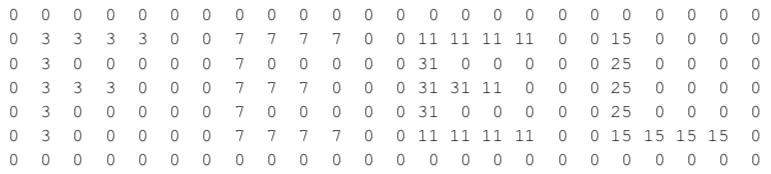
\includegraphics[scale=0.5]{evaluation/File.png}
    \caption{Representation of the file used for simulation}
    \label{file}
\end{figure}

\section{Test post sintesi}
Non è stato possibile sintetizzare il componente e in figura \ref{error_message} è riportato il messaggio di errore. Nonostante questa problematica il componente è in linea di principio sintetizzabile e nessuna istruzione non sintetizzabile è stata utilizzata.

\begin{figure}
	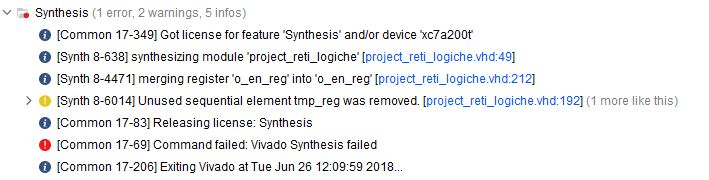
\includegraphics[]{evaluation/error_message.JPG}
    \label{error_message}
    \caption{Syntesis error message}
\end{figure}

